\section{Introduction}

% Motivate need for new process
The Haber-Bosch process for thermochemical synthesis of ammonia from nitrogen and hydrogen transformed the global fertilizer industry and was a critical enabler of the continued expansion of human populations \cite{Smil_1999}. The process is an impressive feat of modern chemical engineering, producing around 150 million tons of ammonia per year at a thermodynamic efficiency of up to 70\% \cite{Schloegl_2003,Schiffer_2017}. However, the process also has downsides. The scale of the process leads to massive energy consumption of 2.5 exajoule per year, and the hydrogen feedstock is typically obtained via methane reforming, leading to a tremendous carbon footprint of 340 Mt of CO$_2$ equivalent per year; this is the highest impact of any commodity chemical production \cite{Schiffer_2017}. Furthermore, the high temperatures ($\sim$700 K) and pressures ($\sim$100 bar) lead to substantial capital cost and favorable economies of scale, driving highly centralized production. This is in contrast to the decentralized use of ammonia-based fertilizers (Fig. \ref{fig:usemap}), which results in substantial transportation costs and additional emissions \needcite. This is particularly impactful in remote locations such as sub-Saharan Africa, where soils are often nutrient-limited due to lack of access to fertilizers\cite{Gilbert_2012, Mueller_2012}. The opposite problem of over-fertilization also has a substantial environmental impact in more developed nations due to the periodic application of highly concentrated fertilizers that cause nitrate pollution in groundwater through leaching. Finally, the intense conditions and reactive nature of concentrated ammonia based fertilizers lead to safety and national security concerns, as evidenced by massive explosions at fertilizer plants and the common use of fertilizers in makeshift explosives.\cite{Marlair_2005}

\begin{figure}
    \centering
    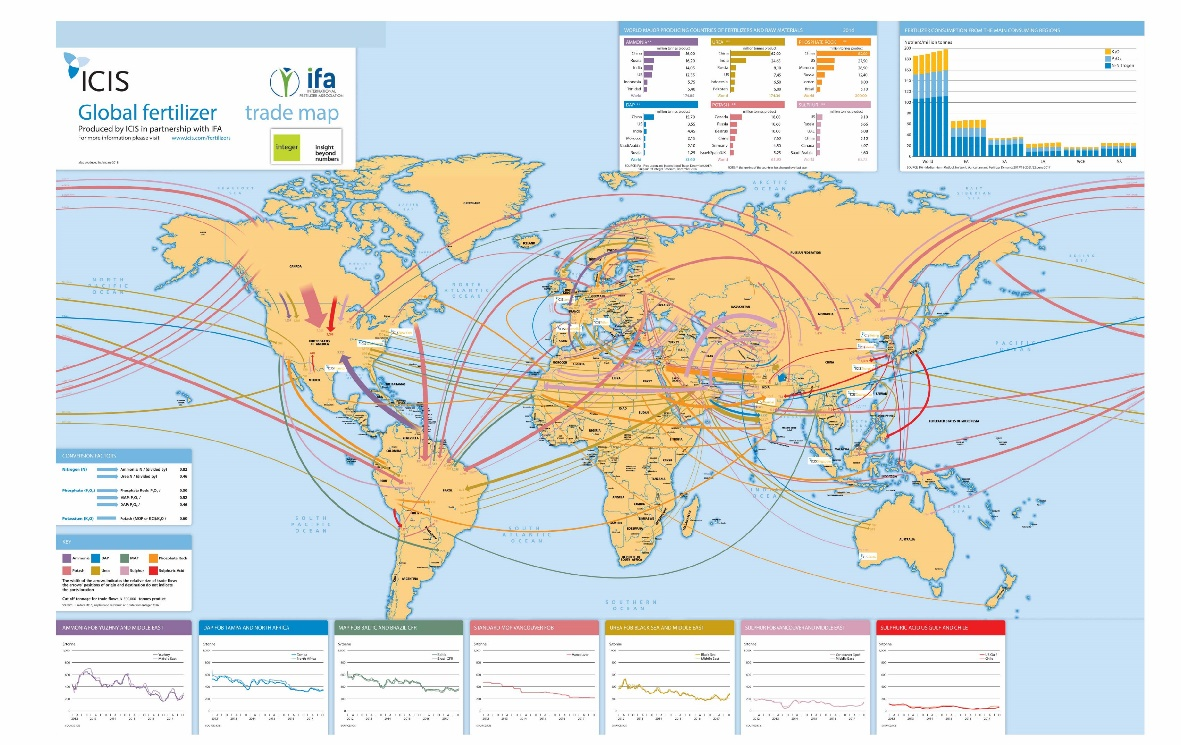
\includegraphics[width=1\textwidth]{Figures/decentralization.jpg}
    \caption{\hl{placeholder figure for illustration of decentralization. Overlay fertilizer use with locations of ammonia plants. Possibly include solar flux map.}}
    \label{fig:usemap}
\end{figure}


% Motivate solar fertilizers
One possible strategy to overcome these disadvantages is decentralized production of aqueous fertilizers using solar energy. These ``solar fertilizers'' could harness solar energy, nitrogen, and water/oxygen from the air to produce lower-concentration ammonia- or nitrate-based fertilizers at or near the point of use. This is advantageous from the perspective of solar energy capture since the intermittent energy is directly captured in a storable product that can be utilized near the point of production, avoiding issues with electricity storage and transport \cite{MacKay_2013}. There are also advantages from an agricultural perspective, since inexpensive feedstocks and reduced transport costs may significantly improve access to fertilizers in remote and developing regions, and the use of lower-concentration fertilizers may also enable novel strategies of nutrient management that can reduce groundwater pollution. Further, low-concentration aqueous fertilizers produced at ambient conditions are inherently safer both from the perspective of the process and the product. Although fertilizers ultimately require a range of nutrients including N, P, and K, the key challenge lies in the fixation of nitrogen and hence this work is focused solely on nitrogen-based fertilizers. Development of solar-driven nitrogen fixation would likely serve as a driver for the development of solar technologies for other nutrients.\hl{This is a little awkward, but we need to point out somewhere that we are only considering N2 fixation here.}

% Motivate need for collaboration with agriculture/fertilizer
Solar fertilizers hold substantial promise as a route to solar energy capture and sustainable agriculture, but there are also considerable challenges. One critical and obvious challenge is in the development of a viable strategy for efficiently using solar energy to dissociate the strong dinitrogen triple bond at ambient conditions. Nitrogen fixation at ambient conditions is a holy grail of chemistry, and has been the subject of considerable research in homogeneous catalysis, enzyme catalysis, and bioengineering, yet no viable strategies have emerged due to issues with low conversion and/or stability under realistic conditions \cite{Vicente_2017,Bur_n_2017,MacLeod_2013,Foster2018}. %need more citations here.
More recently there has been a surge of interest in photo- and electrocatalytic nitrogen fixation by heterogeneous catalysts \cite{Medford_2017,Kyriakou_2017}\needcite. This route is particularly interesting from the perspective of solar fertilizers since photoelectrochemical systems interface will with solar energy, have the potential to scale relatively easily, and have been the subject of considerable research in the solar fuels community.\cite{Kondratenko2013} However, further work is needed to improve the yield and efficiency of photo- and electrochemical nitrogen fixation. %In this work we focus on photo(electro)chemical routes to solar fertilizer production and seek to identify targets and strategies for future research.

Solar fertilizers are also expected to differ significantly from traditional fertilizers, opening a range of additional agronomic challenges. One key difference is that solar fertilizers are expected to have considerably lower fixed nitrogen concentrations, owing to the fact that photo(electro)chemical nitrogen fixation efficiencies are unlikely to compete with the 70\% efficiency of the Haber-Bosch process.\cite{Schloegl_2003} %cite selectivity challenge papers?
Separating and concentrating the ammonia would be energy intensive and likely require centralized facilities, potentially mitigating the advantages of decentralized solar fertilizer production. Direct utilization of dilute fertilizers would avoid or reduce the amount of energy needed for separation/concentration, and may also enable more controlled nutrient management. However, this represents a paradigm shift in agricultural practice, and considerable effort is needed to understand how dilute solar fertilizers can be sustainably and practically integrated with agricultural systems. These considerations will also inform the development of the photo(electro)catalytic processes for solar fertilizer production, and hence should be considered in parallel.

In this work we identify key considerations and performance targets for the photo(electro)chemical production of dilute solar fertilizers from the perspective of catalysis and agronomics. Some specific advantages and disadvantages of decentralized and dilute fertilizer production are outlined and the potential agronomic impacts of varying levels of decentralization are examined. Initial quantitative performance targets are identified based on back-of-the-envelope calculations and possible agricultural scenarios. Finally, the tradeoffs between photo- and electrochemical routes to solar fertilizers are briefly discussed, and some basic reactor design concepts are outlined. We hope that these considerations will serve as a foundation and guide for future research in the development of photo(electro)chemical processes for solar fertilizer production.
%Key considerations are outlined, and several quantitative targets are identified. These targets are preliminary due to the nascent stage of solar fertilizer research, but will provide a starting point for future refinement as the field develops. 

\section{Decentralization of Fertilizer Production}

The price of fertilizer is controlled by a complex interplay of geopolitical and economic factors, particularly the price of natural gas (see Figure \ref{fig:gas_vs_fert}) \needcite. A detailed analysis is beyond the scope of this work, but we briefly introduce some key concepts. The cost of fertilizers can be broken down into production, transportation, and storage. The production cost of fertilizer is controlled primarily by the cost of natural gas used to produce hydrogen for the Haber-Bosch process, and hence varies with location and geopolitical factors. This leads to variable and uncertain cost of fertilizers, leading to challenges in agricultural planning \needcite. This dependence on natural gas also promotes centralized production, with most fertilizer plants located near natural gas deposits \cite{McArthur_2017}. Furthermore, the cost of transportation is highly variable depending on location. Transportation costs as low as ??? \% in the U.S. where ammonia pipelines and railroads connect fertilizer production facilities along the Gulf of Mexico to the agricultural centers in the Midwestern states, or as high as 30\% in landlocked sub-Saharan African countries such as Mali where fertilizers must be transported via ships to a port and subsequently via trucks to agricultural centers \cite{Wanzala2013}. For countries without large-scale fertilizer production it is common to separate transportation costs into domestic and international, since international transportation is more expensive and sensitive to political factors such as tariffs. Finally, the cost of storage must also be considered, although it is generally less variable than transportation or production. \hl{(??? no idea if this is true - the breakdown of production, transport, and storage is hard to find. Let's ask IFDC for a source)} Figure \ref{fig:cost_pies} shows a comparison of the percentage of fertilizer cost arising from each category in 2 representative countries, illustrating the considerable economic impact of fertilizer transportation in the developing world.

\begin{figure}
    \centering
    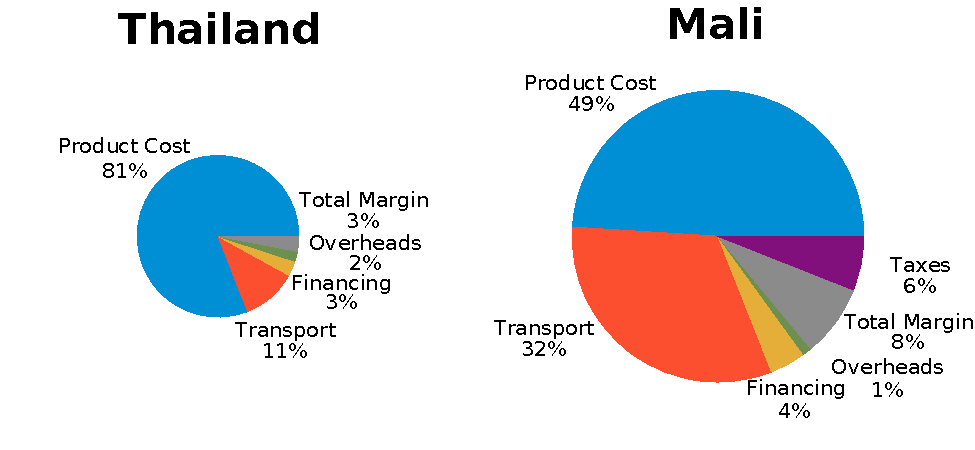
\includegraphics[width=1\textwidth]{Figures/Cost_Breakdown.pdf}
    \caption{The price breakdown for fertilizer in (a) Thailand and (b) Mali for the year 2013. Relative areas reflect the ratio of costs in the two countries (\$282 in Thailand and  \$509 in Mali) numbers from IFDC\cite{Wanzala2013} \hl{we can select different countries and/or add more. Would be interesting to include the US.}}
    \label{fig:cost_pies}
\end{figure}

The total price of fertilizer is not derived directly from its components. For example, the price of fertilizer in Thailand (\$ 287/ton) is roughly half the price of fertilizer in Mozambique (\$ 567/ton), but this difference cannot be attributed directly to any single category. One critical factor that controls this overall price is economy of scale. Developing nations in Africa are often purchasing smaller quantities of fertilizer from the international market, leading to a limited ability to bargain for lower wholesale prices.\cite{Wanzala2013} Larger agricultural markets such as Asia are able to more effectively distribute fixed costs of transportation and negotiation across more units of fertilizer, translating to lower prices at the farm scale. This scale-up is not possible in less developed markets for a variety of reasons including port capacity and poor transportation infrastructure. Political instability often compounds this problem by causing existing infrastructure to deteriorate due to lack of use. Less developed markets are also subject to more uncertain demand owing to lack of access to capital by smallholder farmers and unpredictable implementation of government subsidies. Overall, these factors lead to the perverse situation in which fertilizers are most expensive in the poorest places where the need is greatest. This is a key factor in the distressing fact that despite the tremendous technological developments of the recent decades, world hunger is currently increasing with over 800 million people suffering from undernourishment as of 2016 \cite{FAO_2017}.

Notably, many of these economic and geopolitical factors could be alleviated by decentralized fertilizer production from renewable resources. Lack of dependence on natural gas would reduce volatility in fertilizer production costs, whose prices are highly correlated (see Figure \ref{fig:gas_vs_fert}), and producing fertilizer at or near the point of use would reduce transportation costs and reduce the price dependence on economies of scale. Furthermore, local production would improve certainty in fertilizer availability and reduce the influence of external factors such as tariffs and subsidies. Agricultural production has also been tied to general economic prosperity, and local fertilizer manufacturing industries in developing countries could spur substantial economic growth \cite{McArthur_2017}.
\begin{figure}
    \centering
    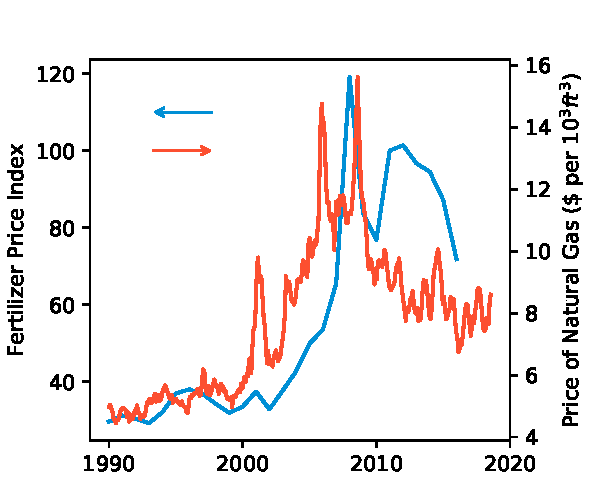
\includegraphics[width=0.7\textwidth]{Figures/gas_vs_fert.pdf}
    \caption{The cost of natural gas paid by industrial consumers in the United States and the price index of fertilizer between over time (www.eia.gov and usda.gov)}
    \label{fig:gas_vs_fert}
\end{figure}
The concept of decentralization is difficult to quantify in general \cite{Schneider_2003}, but in this context we propose the decentralization should scale directly with the total number of fertilizer production facilities. It is useful to examine order-of-magnitude estimates of these quantities to assess the prospects of decentralization. A recent report identified a total of 63 major fertilizer production facilities based on data from the 10 largest producers of ammonia-based fertilizers \cite{McArthur_2017}. While this list may be incomplete, it is expected to be on the correct order of magnitude. This should be normalized by the total agricultural output, which we propose can be estimated by the total number of farms or the total amount of arable land. Both numbers are difficult to know exactly, but a 2014 report estimated the total number of farms to be in excess of 570 million with a total area of around 4.9 billion hectares (another FAO document said 1.5 billion ha) as of 2010 \cite{FAO_2014,Lowder_2016}. This indicates that a single ammonia-based fertilizer plant serves on the order of 10 million farms, or 100 million \hl{(24 million)} hectares of arable land (see Figure \ref{fig:map}) \hl{We need to refine these estimates and ensure that the 4.9 billion number does not include grazing land. The map is based off the smaller number of 24 million based on this source: https://ourworldindata.org/yields-and-land-use-in-agriculture.}.
\begin{figure}
    \centering
    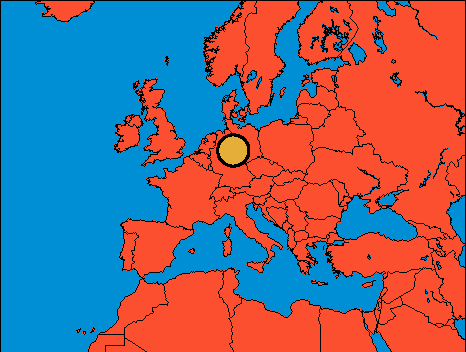
\includegraphics{Figures/approx_size.pdf}
    \caption{The approximate area of land fertilized by an average single Haber-Bosch plant based on rough estimates above. \hl{Revise as needed based on data estimates.}}
    \label{fig:map}
\end{figure}
There are a continuum of options for moving away from this highly centralized scenario. The most extreme alternative would be fully-decentralized ``farm-scale'' fertilizer production, corresponding to roughly 1 fertilizer production facility per farm (or per $\sim$10 ha)\hl{only 3\% of farms are larger than 10 ha per FAO report - we may want to revise this down}, an increase of $\sim$ 7 orders of magnitude in the total number of fertilizer production facilities. This would also correspond to proportional decrease in the scale of production. The global average nutrient load needed for fertilization is $\sim$ 50 kg-N/(ha yr) \needcite \hl{FAO data}, 
corresponding to a capacity of $\sim$ 500 kg-N/yr for farm-scale production. This can be used to estimate the annual revenue expected based on the cost of fertilizer per country. 
In this case, the economic incentives favor decentralized production in countries with high fertilizer prices. 
\hl{Include figure with an overlay the map below with the locations of the N fertilizer plants (Both data are openly available) http://sedac.ciesin.columbia.edu/downloads/maps/ferman-v1/ferman-v1-nitrogen-fertilizer-application/nitrogen-fertilizer-global.jpg (here or in the introduction? Currently Fig. 1)}
For example, the price of urea in Ghana in 1999 was approximately \$1100/MT, or \$ 2350/MT-N (urea is 46\% N by weight). \hl{These numbers need to be cleaned up}
This corresponds to an expected annual revenue on the order of \$ 1200/year. This relatively modest number suggests that fully decentralized fertilizer production must have very low capital and operating costs, even in countries where the cost of fertilizer is very high. Furthermore, the process must be sufficiently robust that specialized operators are not needed for operations or maintenance. This suggests that ``frugal innovation'' strategies \cite{Weyrauch_2016} may be required for the development of inexpensive and robust processes for farm-scale fertilizer.

Less extreme alternatives would be ``small-scale'' or ``medium-scale'' fertilizer production facilities, which could serve on the order of 100 or 10,000 farms respectively. As production becomes more centralized the economics will favor more capital investment and labor specialization, enabling development of more technically advanced processes. The small-scale facility would have a production capacity of 50 MT-N/yr, while a medium-scale facility would produce 5,000 MT-N/yr. Assuming capital costs similar to current ammonia production are economical ($\sim$ \$1,000/MT-N), this corresponds to \$50,000 or \$5 M of capital expense, which is rather modest by the standards of chemical plant construction. Other scales are also possible, and we propose the following relationship between capital cost and area of arable land served: $C_{capital} \approx \$ 50 \times A_{arable}$ where $C_{capital}$ is capital investment in dollars and $A_{arable}$ is the arable land area in hectares. This analysis is overly simplistic this will vary considerably depending on the market price of fertilizer and the cost of operators, feedstock, and maintenance; however, it can provide an order-of-magnitude estimate regarding the type of process that may be feasible to serve a specific amount of land, or conversely the scale needed for a process given an estimate of capital investment. For example, electrochemical processes are likely only feasible at small or medium scales, while photochemical processes may be possible at the farm scale. This is discussed further in Section \ref{sec:approaches}. \hl{This analysis is clearly naive and incomplete. It would be great to expand this to get estimates of operational and labor costs for photo/electrochemical processes if possible. We should try to determine a clearer scope based on the numbers we think we can come up with.}

\section{Dilute fertilizers}

The centralized production of fertilizers along with the high purity of Haber-Bosch ammonia has driven the development of fertilizers with high weight percent nitrogen (35-85\%) to reduce transportation and storage costs. This is in contrast to the biological production of nitrogen that occurs directly in the root system of the plants and results in relatively low local concentrations of fixed N in the soil \needcite \hl{Some more details/numbers here might be nice.}. The prospect of decentralized fertilizer production thus also enables the possibility of the production of dilute fertilizers, since transportation and storage costs can be minimized or eliminated if fertilizers are produced on-demand at the point of use. Utilization of solar energy is expected to produce fertilizers with much lower nutrient densities owing to the lower density of solar energy \needcite and the challenges with low efficiency and selectivity in photo(electro)chemical nitrogen fixation. As discussed in Section \ref{sec:targets} the required solar-to-ammonia efficiencies and nutrient concentrations are in principle surprisingly low; however, these low-concentration fertilizer products differ substantially from existing fertilizers and present a number of challenges. As discussed in the Section \ref{sec:targets} we estimate that the dilute limit for fertilizers is $\sim$1 wt\%-N in aqueous solution, although $\sim$3-5 wt\%-N is likely necessary for practical relevance since when solar radiation, temperature, and soil water availability are non-limiting, plant nutrient requirements will be higher. This is in contrast to typical solid urea fertilizers that are 47 wt\%-N, and hence much more economical to transport. For small- or medium-scale production it would likely be necessary to separate or concentrate the fixed-N product to concentrations comparable with existing products (20-40 wt\%-N) for transport or storage. This additional separation process would require further capital investment and operational costs. However, in the limit of farm-scale decentralization transportation may be less of an issue, since dilute fertilizer could be directly applied through irrigation systems. Even at the farm-scale such dilute fertilizers would present challenges with storage, and an irrigation system would be required for application. The latter is a particular challenge for many smallholder farms in sub-Saharan Africa, where only around 7\% \hl{IFDC number from C. Dimkpa} of farms are equipped with irrigation \needcite. Nonetheless, these farms still present a sizable market, and the prospect of combined fertilization/irrigation systems may favor investment in irrigation systems. \hl{It would be good to come up with some estimates of cost for transportation/storage as a function of dilution (volume).} Furthermore, electrochemical systems that can operate from the electricity grid could be used to produce dilute fertilizers on demand, mitigating the need for storage costs. This technology may be useful in more developed countries where farms for many crops have existing irrigation systems.

One enticing possibility for dilute fertilizers is the prospect of improved nutrient management. Currently the fixed nitrogen in fertilizers is not utilized efficiently, with 20-50\% being lost to leaching or vaporization.\hl{Expand discussion here?} \needcite This is more prevalent in developed countries where fertilizers are inexpensive, and particularly in the case of potent anhydrous ammonia fertilizers \needcite \hl{This is an assumption, but we need evidence}. These highly concentrated fertilizers release nutrients too rapidly for plant uptake. Not only is this inefficient, but it also results in pollution of groundwater by nitrates and release of N$_2$O, one of the most potent greenhouse gases. The most common strategy for mitigation of these effects is the development of coatings that aid in controlled release of nutrients and enhance uptake efficiency \hl{Not sure about this. Are there other approaches to mention here? Are fertilizers already applied in irrigation sometimes? Are other fertilizers than urea (e.g. calcium ammonium nitrate) used for this?}. While effective, the use of dilute fertilizers offers a different approach in which nutrients are delivered at a controlled rate. This would enable matching N supply with crop demand, and However, substantial additional research into agronomics and plant nutrition is required to determine the potential of this strategy and identify the optimal nutrient concentration and application profile. Another advantage of dilute fertilizers are their inherent safety since they will be less corrosive and more difficult to convert into explosives. These factors suggest that further research into the utility and effectiveness of dilute fertilizers is relevant to the field of solar fertilizers.

\section{Preliminary Performance Targets}
\label{sec:targets}

There has been a substantial recent increase in photo(electro)chemical nitrogen fixation research, yet there are no targets for how efficient these processes need to be. In this section we briefly outline targets for solar-to-ammonia efficiency, total fixed nitrogen concentration, and required rates of nitrogen fixation that have the potential to enable solar fertilizer production. These targets are not meant to be authoritative, but rather provide guidelines for catalyst development and fertilizer testing. 

One key consideration is the overall efficiency required to convert solar energy to fertilizer. First, we estimate the areal energy density required for fertilization based on an assumption of 50 kg-N/(ha yr) provided by ammonia-based fertilizers:
\begin{equation}
\mathrm{
50 \frac{kg_N}{ha . yr} \times \frac{10^3}{14} \frac{mol_{NH_3}}{kg_N} \times \frac{667}{2} \frac{kJ}{mol_{NH_3}} \times \frac{1}{10^4} \frac{ha}{m^2} \times \frac{1}{3.15e7} \frac{yr}{s} = 3.77 \frac{mW}{m^2}
}
\end{equation}
this remarkably low energy density is roughly 6 orders of magnitude below the solar constant of 1000 W/m$^2$, indicating that high efficiencies are not necessary. An initial estimate can be obtained by assuming 8 hours of full sunlight per day and 1\% of arable land dedicated to solar capture \cite{Medford_2017}. In this case the average solar flux is 333 W/m$^2$ and the corresponding required solar-to-ammonia efficiency is $\sim$0.1 \%. Data on actual average solar fluxes reveals that they vary from 120 - 280 W/m$^2$ depending on latitude \cite{MacKay_2013}, and there is also considerable variability in the nutrient load required, ranging from 15-200 kg-N/m$^2$ depending on a myriad of factors including crop and soil type \needcite. Based on these estimates the required solar-to-ammonia efficiency may range from 0.05 - 1.25 \% depending on solar flux and required nutrient load. These estimates assume that 1\% of arable land is dedicated to solar capture, and will vary linearly with the percentage of land available. We propose that 1\% is a relatively conservative number, corresponding to 100 m$^2$/ha or roughly 6 typical solar panels per hectare \needcite. Notably, solar-to-ammonia efficiencies as high as 0.02 \% have been reported for nitrogen fixation photocatalysts, suggesting that the efficiency target is feasible with further research.

In addition to efficiency it is also critical to consider the concentration of fixed nitrogen needed for a product to be considered a fertilizer. The limiting case can be determined by assuming that the nutrients will be included directly in the irrigation lines. However, the amount of irrigation needed is highly variable depending on crops, rainfall, location, and socioeconomic factors (http://www.fao.org/docrep/u5835e/u5835e04.htm). Nonetheless, we propose an estimate of 1500 L/ha/y as a typical number for practical scenarios. Further, we note that while 50 kg-N/(ha yr) is a typical nitrogen nutrient load, the critical lower boundary for nutrient consumption can be as low as 15 kg-N/(ha yr). From these estimates we propose a lower boundary of 1 kg-N/L, or 1 wt \% N, as a convenient estimate for the minimum nitrogen concentration that can be considered a fertilizer \hl{compare to aqua ammonia and potential get insight from IFDC on what the potential impact might be of these low loads. Any previous experience where aqua ammonia is used for direct application?}. This is roughly 1 order of magnitude lower than existing aqueous fertilizers, but it is 5-8 orders of magnitude above the concentrations reported for typical photo(electro)chemical nitrogen fixation processes where yields are typically reported in units of $\mu$M or mM. This large gap between the proximity of efficiency and concentration targets is due to a combination of large water volumes and the short testing times that are typically employed for photo(electro)catalysts. Photocatalytic ammonia production is often measured in the gas-phase, where ammonia sticks to the catalyst surface and must be washed off with large volumes of water, leading to low concentrations, and in aqueous photo(electro)chemical settings the fluid volumes are typically on the order of 100mL while illumination areas are on the order of cm$^2$. Furthermore, testing times on the order of days to weeks are considered long by academic standards. This leads to extremely low concentrations that are outside of the regime that can be considered fertilizer. Operating the catalysts in higher ammonia concentration regimes may impact the performance of the process, suggesting that future efforts should focus on designing cells and testing procedures that lead to substantially higher concentrations. These higher concentrations lead to an additional advantage for analytical characterization, since difficulties in quantifying ammonia at nM - $\mu$M concentrations have plagued the field. As concentration increases the issues with contamination will be less prevalent, and the presence of ammonia should become unmistakable due to its pungent odor that can be detected with concentrations as low as 50 ppm (equivalent to 3 mM in the aqueous phase).

A further consideration that is particularly relevant to electrochemical ammonia production is the current densities that are required for practical operation. In the case of solar fuels the overpotential for oxygen evolution has been defined as the potential at which the current is equal to 10 mA/cm$^2$, equivalent to 10 \% solar-to-fuel efficiency. In the case of solar fertilizers the necessary current will be substantially lower, due to the substantially lower solar-to-ammonia efficiency requirements. For simplicity, we will assume that a 0.1\% solar-to-ammonia efficiency is required. However, an additional consideration that is more relevant for electrochemical nitrogen fixation is the Faradaic efficiency that governs the selectivity to ammonia (or nitrates) over other possible products. Indeed, low selectivity to ammonia due to hydrogen evolution has proven to be a critical challenge for electrochemical ammonia synthesis. Typical reported ammonia selectivities are $<$ 1\%, although several recent reports have achieved Faradaic efficiencies on the order of 10 \%. By assuming 10 \% Faradaic efficiency and an overall solar-to-ammonia efficiency of 0.1 \%, the relevant current density is 1 mA/cm$^2$. Notably, Faradaic efficiency is often a strong function of applied potential (and the resulting current density), with high Faradaic efficiencies typically corresponding to very low current densities on the order of nA/cm$^2$ - $\mu$A/cm$^2$. Nonetheless, a recently-reported carbon-based catalyst achieved $>$10 \% Faradaic efficiency at a current density of ca. 4 mA/cm$^2$, indicating that it is possible to achieve high Faradaic efficiencies at the proposed operating current of 1 mA/cm$^2$. Measuring overpotential and Faradaic efficiencies at practical current densities provides a useful route to identifying electrocatalysts that are promising for solar fertilizer production.

\hl{Possible paragraph or table outlining suggested testing standards (temperature, pressure, pH, illumination intensity, etc.) for photo- and electrochemical approaches?}

\section{Approaches for Solar Capture}
\label{sec:approaches}

The solar fuels community has identified two basic strategies for conversion of solar to chemical energy: direct capture of photons through photochemistry, or indirect capture through photovoltaics coupled to electrochemistry.\cite{McDaniel_2010,Highfield_2015} The hybrid approach of photoelectrochemistry, where electrical bias is applied in conjunction with solar capture has also been explored. There has been considerable debate and analysis regarding the efficacy of these approaches for fuel production \hl{(studies by Jaramillo, Lewis, others)}, and while there is no clear consensus the indirect capture route has received considerable attention. While some of the same considerations apply to the case of solar fertilizers, there are also a number of key differences. In particular, the concentration/efficiency requirements are much lower for fertilizers, and the products are considerably less volatile. While a detailed technoeconomic analysis is beyond the scope of this work, we present some general considerations for each approach.

\hl{Include a figure here similar to the figures in solar fuels papers (e.g. Nate Lewis' work) comparing these two approaches}

The direct capture of photons and conversion to fertilizer is the most straightforward and decentralized route to solar fertilizer production. Direct capture typically involves a single catalytic material (or composite catalyst) that could be produced in massive quantities and distributed to remote locations. It is possible to envision relatively simple reactor designs that could be integrated directly with an irrigation system and not require specialized labor. These systems could be designed without toxic electrolytes, avoiding the need for an additional separation process, and opening the possibility of inexpensive solar fertilizer reactors that could be deployed at the farm scale. However, the concentration of nutrients will be limited by the solar flux, leading to substantial uncertainty and likely lower concentrations. Furthermore, photochemical technologies are relatively untested, and there is currently no catalyst capable of the required solar-to-ammonia efficiency of 0.1 \%. The most widely-used photocatalysts are for environmental applications such as reducing contamination or self-cleaning glass where concentrations are low and catalysts are inexpensive. It is possible to envision solar fertilizer schemes that are similar to these environmental applications, but they would likely require close integration with agricultural infrastructure. For example, farms where irrigation is heavily employed are good candidates for direct solar fertilizers, particularly if they are located in remote regions. Roughly 7\% of farms in sub-Saharan Africa make use of irrigation. This is far from a majority, but still represents a substantial agricultural footprint where direct photochemical fertilizers might have a practical impact.

The alternative approach of capturing solar energy with photovoltaics and subsequently producing electrochemical ammonia also has a number of advantages. Photovoltaic technology is well-established, and efficiencies of 10-20 \% are typical. This leads to a required electrical-to-ammonia efficiency of $\sim$ 1\%, which is relatively low and has been reported at the lab scale for state-of-the-art ammonia electrocatalysts. Furthermore, electrochemical technologies have been demostrated at scale, including the chloroalkali process, water hydrolysis, and hydrogen fuel cells \needcite. Electrochemical fertilizer production can be integrated with an electrical grid, providing reliable yields even in periods of no sunlight and the use of high current densities can enable the production of high concentrations of fixed nitrogen. However, large-scale electrochemical processes are far more complex than direct photocatalysis, and may require larger-scale facilities and specialized labor. In addition the practical efficiencies of solar cells on a per-area basis are much lower than their theoretical efficiencies, particularly if they are not installed with advanced technologies such as solar tracking, increasing the capital and labor requirements \needcite \hl{McKay paper}. Electrochemical processes also require electrolytes to provide electrical conductivity and control the pH. Some reports have indicated that Li-based electrolytes exhibit high performance for electrocatalytic nitrogen reduction to ammonia \needcite \hl{Rondinone paper, others?}. In general the effect of electrolytes on plant growth are unknown, and some electrolytes that contain metals such as Li can be costly, indicating that separation of electrolytes may be required. On the other hand, many electrolytes such as NaCl are abundant and non-toxic, while others such as KOH and Na$_2$H$_2$PO$_4$ could provide an additional source of nutrients if they are not separated. Nonetheless, the need to deal with electrolytes introduces an additional engineering challenge. These intensive production processes would lead to higher capital costs and more centralized production; in this case issues with fertilizer transport would become relevant. As centralization increases the process will be in more direct competition with the established Haber-Bosch process, and more detailed technoeconomics will be necessary to determine if such an approach is competitive. Nonetheless, the scale of electrochemical processes is still expected to be orders of magnitude below Haber-Bosch, and the process is likely to be less capital-intensive and more robust to uncertainty in electrical power. This suggests that agricultural areas in developed countries, near medium or large cities, or in land-locked areas are most promising for indirect capture of solar energy and subsequent electrochemical conversion to fertilizers.

\hl{Add a table here with properties/advantages/disadvantages of direct vs. indirect?}

\section{Conclusions}

Solar fertilzers present an exciting opportunity to directly capture diffuse solar energy and convert it to chemical energy that can be applied at or near the point of production. The technology falls at the complex nexus of energy and agriculture, and substantial additional research is needed to establish the most promising approaches and demonstrate the technology. This work grapples with some initial considerations from the perspective of agronomics and photoelectrochemistry, and identifies some preliminary metrics that will aid in the development and deployment of solar fertilizer technologies. Specific metrics are presented to identify the target solar-to-ammonia efficiency (0.1\%), minimum nitrogen concentration (1 wt\%), and electrochemical current density (1 mA/cm$^2$) that may enable solar fertilizer technology, and considerations for assessing direct and indirect capture and conversion of solar energy are presented. The metrics and considerations presented draw on a range of expertise in the diverse fields of agronomics, photoelectrocatalysis, and process systems engineering, and provide a starting point for further development of solar fertilizer technologies. There are many possible routes forward for this nascent field, and identifying the most promising will require a diverse range of technical, social, and economic considerations. However, the vast potential impact of solar fertilizers on the growing problem of world hunger makes this challenging endeavor worthwhile.


